%----------------------------------------------------------------
%
%  File    :  thesis.tex
%
%  Authors :  Wolfgang Radinger-Peer
% 
%  Created :  03 Feb. 2019
% 
%  Changed :  03 Feb. 2019
% 
%----------------------------------------------------------------

% --- Document Definition  ----
\documentclass[11pt,a4paper,oneside]{scrbook}

% language definition
\usepackage[english]{babel}

%\usepackage{lmodern}

\usepackage[T1]{fontenc}

% Font definition
\usepackage{helvet}
\renewcommand{\familydefault}{\sfdefault}

\usepackage[bf,sf]{subfigure}
\renewcommand{\subfigtopskip}{0mm}
\renewcommand{\subfigcapmargin}{0mm}

\usepackage{url}

% Package for formulas 
\usepackage{mathtools}

\usepackage{latexsym}

\usepackage{ifpdf} % detect outputstyle

\usepackage{geometry} % define pagesize in more detail

% Package for header and footer 
\usepackage{fancyhdr} 
\renewcommand{\footrulewidth}{0.4pt}

% Package for colored backgrounds for tables
\usepackage{colortbl} 

% Package for colored source code listings
\usepackage{courier} 
\usepackage{listings} 
\lstset{basicstyle=\ttfamily,breaklines=true}

% Package for pdf generation
\usepackage[pdftex]{graphicx}
\DeclareGraphicsExtensions{.pdf,.jpg,.png}
\pdfcompresslevel=9
\pdfpageheight=297mm
\pdfpagewidth=210mm
\usepackage[         % hyperref should be last package loaded
    pdftex,
    bookmarks,
    bookmarksnumbered,
    linktocpage,
    %pagebackref,
    pdfview={Fit},
    pdfstartview={Fit},
    pdfpagemode=UseOutlines,                 % open bookmarks in Acrobat
  ]{hyperref}
\usepackage{bookmark}

\geometry{a4paper,left=30mm,right=25mm, top=30mm, bottom=30mm}

% to set the path for figures and examples
\graphicspath{{figures/}{examples/}}

% vert. space before a paragraph
\setlength{\parskip}{3pt plus 1pt minus 0pt}      
\setlength{\parindent}{0pt}

% Definition of the table of contens
\setcounter{tocdepth}{2}          % lowest section level in TOC
\setcounter{secnumdepth}{3}  % lowest section level still numbered

% Bibliography style
%\usepackage{apacite}
%\usepackage[nottoc,numbib]{tocbibind}
%\renewcommand{\tocbibname}{\textsc{Bibliography}}

% Biblatex
\usepackage[style=apa]{biblatex}

% --- Start of Document ----------------------------------------
\begin{document}
\linespread{1.3}
\frontmatter
\normalsize

\pagestyle{empty}      % for title pages
%----------------------------------------------------------------
%
%  File    :  title.tex
%
%  Authors :  Wolfgang Radinger-Peer
% 
%  Created :  03 Feb. 2019
% 
%  Changed :  03 Feb. 2019
% 
%----------------------------------------------------------------

% MODUL University logo
\begin{picture}(50,50)
\put(+300,40){\hbox{\includegraphics{header.png}}}
\end{picture}

\hspace*{-1.0cm} {\huge \textbf{<Title of the Master Thesis> }}

\vspace{0.2cm}
\noindent\makebox[\linewidth]{\rule{18cm}{0.4pt}}
\vspace{1cm}

\hspace*{-1.0cm} {\Large Master Thesis submitted in fulfillment of the Degree}
\vspace{0.4cm}

\hspace*{-1.0cm} {\Large Master of Business Administration}
\vspace{0.4cm}

\hspace*{-1.0cm} {\Large in <Study Program>}
\vspace{2.2cm}

\hspace*{-1.0cm} Submitted to <Name of Supervisor>
\vspace{2.2cm}

\hspace*{-1.0cm} <Name of Author>
\vspace{0.65cm}

\hspace*{-1.0cm} <Student number>
\vspace{2.2cm}

\hspace*{-1.0cm} Vienna, {\today}
\vspace{0.2cm}
              % Title Page

% style for the for preliminary pages
\pagestyle{fancy}
\fancyhead{}
\fancyfoot{}
\setlength{\headheight}{15pt}
\renewcommand{\headrulewidth}{0.0pt}
\fancyfoot[R]{\thepage}      
\pagenumbering{Roman} 

% --- Affidavit ----------------------------------------------------
\cleardoublepage
\setcounter{page}{1}
\addcontentsline{toc}{chapter}{Affidavit}         
%----------------------------------------------------------------
%
%  File    :  affidavit.tex
%
%  Authors :  Wolfgang Radinger-Peer, MODUL University Vienna
%		     based on FH Campus Wien, Austria 
%
%  Created :  1. Feb 2019
% 
%  Changed :  1. Feb 2019
% 
%----------------------------------------------------------------

{\Large\textbf{\textsc{Affidavit}}}

I hereby affirm that this Master’s Thesis represents my own written work and that I have used no sources and aids other than those indicated. All passages quoted from publications or paraphrased from these sources are properly cited and attributed.

The thesis was not submitted in the same or in a substantially similar version, not even partially, to another examination board and was not published elsewhere.

\vspace{2.0cm}
\noindent\makebox[\linewidth]{\rule{7cm}{0.4pt}  \hspace{1.0cm} {\rule{7cm}{0.4pt}}}

\hspace{3.0cm} Date \hspace{7.0cm} Signature\\


\newpage 
\quad
\newpage

% --- Abstract ----------------------------------------------------

\cleardoublepage
\addcontentsline{toc}{chapter}{Abstract}           
%----------------------------------------------------------------
%
%  File    :  abstract.tex
%
%  Authors :  Wolfgang Radinger-Peer, MODUL University Vienna
%
%  Created :  1. Feb 2019
% 
%  Changed :  1. Feb 2019
% 
%----------------------------------------------------------------

{\Large \textbf{\textsc{Abstract}}}

\vspace{0.65cm}

A short summary of your thesis, describing the background, your objectives and the most important outcomes, it may also include some of the conclusions of your thesis. 
This template gives an example of how you may organize your thesis, which can be a challenge in itself considering the scope of the project that you now are embarking on. Bear in mind that it is only a suggestion, and that you should adapt this template in the way that you think suits your thesis the best. This template is based on the structure of completed master theses of high standard. The formatting applied to this template is an ex-ample of how you should format your thesis (e.g. use of headings, tables that you need to include etc.)
        

\newpage 
\quad
\newpage  

% --- Acknowledgement ---------------------------------------
\cleardoublepage
\addcontentsline{toc}{chapter}{Acknowledgement}          
%----------------------------------------------------------------
%
%  File    :  acknowledgement.tex
%
%  Authors :  Wolfgang Radinger-Peer
%             
% 
%  Created :  03 Feb. 2019
% 
%  Changed :  03 Feb. 2019
% 
%----------------------------------------------------------------

\cleardoublepage

{\Large \textbf{\textsc{Acknowledgments (Optional)}}}

\vspace{0.65cm}

A list of institutions and people who may have contributed to your thesis, which you think deserve a mention under this heading.

\newpage

  

\newpage 
\quad
\newpage

% --- Table of Contents ---------------------------------------
\renewcommand*\contentsname{Table of Contents}
\setlength{\parskip}{3pt plus 3pt minus 3pt}  
\tableofcontents   % Table of Contents

% --- List of Figures --------------------------------------------
\newpage
%\phantomsection
%\addcontentsline{toc}{chapter}{List of Figures}
\listoffigures

% --- List of Tables ---------------------------------------------
\newpage
%\phantomsection
%\addcontentsline{toc}{chapter}{List of Tables}
\listoftables

% --- Glossary ---------------------------------------
%----------------------------------------------------------------
%
%  File    :  glossary.tex
%
%  Author  :  Wolfgang Radinger-Peer
% 
%  Created :  03 Feb 2019
% 
%  Changed :  03 Feb 2019
% 
%----------------------------------------------------------------

\noindent
{\Large\bfseries \textsc{List of Abbreviations}}
\vspace{0.65cm}

\begin{table*}[htbp]
		\begin{tabular}{ll}
			APA & American Psychology Association\\
			MU & MODUL University\\
		\end{tabular}
\end{table*}

	           

% --- Main Part ---------------------------------------
\mainmatter

\cleardoublepage

% style for the for main pages
\pagestyle{fancy}         
\renewcommand{\headrulewidth}{0.4pt}
\fancyhead[RO]{\slshape \nouppercase{\leftmark}}
\fancyfoot[R]{\thepage}   
\pagenumbering{arabic} 

%--- here start the chapters  ----------
%----------------------------------------------------------------
%
%  File    :  intro.tex
%
%  Authors :  Wolfgang Radinger-Peer
% 
%  Created :  3. Feb 2019
% 
%  Changed :  3. Feb 2019
% 
%----------------------------------------------------------------

\chapter{\textsc{Introduction}}
\label{chap:intro}

An intro that will lead into the theoretical framework which follows in the next chapter

\section{Headings}
\label{sec:heading}

Headings structure a text and demonstrate the importance of individual sections. Different levels of structure must be indicated by different heading levels. 
Paragraphs that are of equal importance receive headings of the same level.

\subsection{Creating headings}
\label{sec:}

The headings in this chapter as well as the other chapters will largely be dependent on your research. The introductory chapter serves as a presentation and an overview of your thesis. You need to make the reader familiar with the topics that you will investigate, and prepare him/her for what is forthcoming throughout the next chapters. 

\section{Formatting throughout the thesis}
This section will describe the formatting that should be applied throughout the thesis.

\subsection{Fonts and alignment}
\label{sec:fonts}
The font used should be consistent throughout the thesis. The default font for Word 2007 is Calibri (11pt) which is accepted, 
as well as other sans fonts such as Arial and Helvetica (11pt). 
Paragraphs should always be separated with a line break (but not with a blank line), and the text should be justified. 

\subsection{Margins and spacing}
\label{sec:margins}

The margins preferred for the thesis are defaults in Word 2007:
\begin{itemize}
\item Left and right margins: 1 inch (2.5 cm)
\item Top and bottom margins: 1 inch (2.5 cm)
\item Back margin: 0.4 inches (1 cm)
\end{itemize}
	
The thesis should have line spacing of: “Multiple 1.3” and a spacing before each paragraph (quick style “Normal”) of 12 pt. 

\subsection{Page numbering and printing}
\label{sec:pagenumbering}

Pages should be numbered throughout the thesis. The page number is on even pages left aligned, on uneven pages right aligned. The thesis should be printed on both sides to save paper. 

\subsection{Referencing in text/citation}
\label{sec:referencing}
The thesis should be fully referenced, and any material used without providing a reference is considered as plagiarism. 
To see the university guidelines on plagiarism, please go to http://www.modul.ac.at/sites/modul/files/Plagiarism.pdf. 
Direct, literal citation is always reproduced to the letter and set in “quotation marks.” As a general rule, longer citations are – if they are absolutely necessary – 
formatted differently for a better accentuation and displayed with an indent. Indirect, analogous reference to citations (“paraphrases”) must also be 
labeled (mainly with “cf.”), since it involves an external body of thought despite there being a description in your own words. The following list serves as a 
guideline about how to quote different sources using APA formatting. 
This system does not use footnotes, but it offers a brief note in the text about where the information comes from. 

The work of an individual author:
... previous pre-occupation with this phenomenon (Müller, 1954) ...
... Müller (1954) already dealt with this phenomenon ...
A particular page or pages should be specified:
... Kristofferson (1990, p. 268) offers an alternative explanation...
... An alternative explanation is offered by Kristofferson (1990, pp. 268-70)....
The work of two authors:
… further analysis (Schmid \& Maier, 1973)…
… according to Schmid \& Maier (1973), …
The work of several authors:
Only the name of the first author is stated, followed by “et al.“ and the year
… Maier et al. (1981)
Several works of different authors:
...This interpretation is disputed by several scholars (O’Keefe 1988; Joye 1989).
Two different works of the same author
... Parton (1991a; 1991b) has carried out a number of research projects which reinforce these findings.
... Parton (1991; 1996) has carried out a number of research projects which reinforce these findings.
Secondary Citations
In the case of secondary citations, the original source is no longer available or accessible. The citation belonging to the author of the original research paper that is no longer avail-able appears in the text followed by parentheses or if this citation is already in parentheses, after a comma followed by the note “cited by” and details of the respective source that is available to the author. However, the original work that is not present must be cited in the bibliography.
… Müller (1954, cited by Barnabas, 1960) 
… (Müller, 1954, cited by Barnabas, 1960)
Internet references
The main rule to remember is that the citation should be matched to the reference in the bibliography. Thus, the citation should be made using the name/organization which is displayed in the bibliography.
… (World Tourism Organisation, 2009). 

\section{Research aims and objectives (and hypotheses if applicable)}
\label{sec:aims}
Aims and objectives should be clearly stated. 

\section{Structure of thesis}
\label{sec:structure}
Under the last heading of the first chapter you should give a short description of the chapter layout of the thesis.


%  \cite{Urstadt:2009aa}        (Urstadt, 2009)
%  \citeA{Urstadt:2009aa}      Urstadt (2009)
%  \citeNP{Urstadt:2009aa}   Urstadt, 2009
% \cite{Bollen:2011aa}		(Bollen & Mao, 2011)
% \citeA{Bollen:2011aa}		Bollen and Mao (2011)
% \citeNP{Bollen:2011aa}		Bollen & Mao, 2011
% \citeyear{Bollen:2011aa}		(2011)
% \citeauthor[p. 5]{Bollen:2011aa}	Bollen and Mao, p. 5

            % Introduction

%----------------------------------------------------------------
%
%  File    :  theorie.tex
%
%  Author :  Wolfgang Radinger-Peer
% 
%  Created :  3. Feb 2019
% 
%  Changed :  3. Feb 2019
% 
%----------------------------------------------------------------

\chapter{\textsc{Literature Review}}
\label{chap:theory}

\section{Introduction}
\label{sec:introcap2}

Overview of chapter and linking with previous chapter

\section{Theoretical framework (if applicable)}
\label{sec:introcap2}

A diagram showing how the different topics within the literature relate, and how they come together in your research

\section{First relevant topic within literature}
\label{sec:rel1}

\subsection{Sub-topic}
\label{sec:rel1sub1}

\subsection{Sub-topic}
\label{sec:rel1sub2}

\cite{Fowler72s}


\section{Second relevant topic... etc}
\label{sec:rel2}

Etc… the number of relevant topics and sub-topics will vary depending on the nature and scope of your research. What is important to remember is that all 
relevant topics should be included in the literature review, and serve as an introduction to your research. Later in the thesis you will refer your findings back to
 relevant literature in this chapter, so it needs to cover all the literature that is of importance to your findings. 
In addition, you should state how your thesis will contribute to the current knowledge, either by making this explicit under a separate heading or by 
mentioning the contribution of the thesis throughout the chapter where relevant additions will be made. 

\section{Conclusion}

Short summary and link to next chapter

       % Theorie

%----------------------------------------------------------------
%
%  File    :  method.tex
%
%  Author :  Wolfgang Radinger-Peer
% 
%  Created :  3. Feb 2019
% 
%  Changed :  3. Feb 2019
% 
%----------------------------------------------------------------

\chapter{\textsc{Methodology}}
\label{chap:method}

\section{Introduction}
\label{sec:introchapter3}
Overview of chapter and linking with previous chapter.

\section{Selection of methodology}
\label{sec:selectionmethod}

Relevant factors which led you to choose this methodology and mention of methods used in previous and relevant research.

\section{Research instrument}
\label{sec:researchinstrument}

Description of the relevant method for collecting data, such as questionnaire, interview schedules etc. (these should be included in the \nameref{chap:app} section). 

\section{Selection of study site (if applicable)}

\section{Pilot tests (if applicable)}

\section{Sampling procedures (if applicable) }

\section{Data analysis}
\label{sec:dataanalysis}

Overview of methods used for analyzing the data, relevant analyses, description of stages in the analysis etc. 

\section{Other relevant topics and headings}
\label{sec:othertopics}

\section{Conclusion}
\label{sec:conclucionchapter3}
\underline{Short} summary and link to next chapter
       % Method

%----------------------------------------------------------------
%
%  File    :  results.tex
%
%  Author :  Wolfgang Radinger-Peer
% 
%  Created :  3. Feb 2019
% 
%  Changed :  3. Feb 2019
% 
%----------------------------------------------------------------


\chapter{\textsc{Results and Discussion}}
\label{chap:results}

\section{Introduction}
\label{sec:introcap4}

Overview of chapter and linking with previous chapter

\section{Visual presentation of the findings}
\label{sec:visualrep}

Findings should be grouped together under relevant headings and discussed accordingly. This means that they should be interpreted and be 
put into the context of previous literature, and findings from other related research. The findings can be presented in a number of ways, 
including tables, graphs, text descriptions and figures. The presentation should be able to communicate the most important aspect of your findings. 
One thing to remember: the figures, tables and graphs should be clearly labelled, numbered and referred to in the text. To achieve a numbering which 
is consistent throughout the thesis you can use captions, and to make it look more professional it is advisable to use the chapter number in the numeration of your visual presentations. 

\section{Tables}
\label{sec:tables}

\section{Usage of tables}
\label{sec:usagetables}

\begin{itemize}
\item The document will be used to look up individual values
\item The document will be used to compare individual values
\item Precise values are required
\item The quantitative information to be communicated involves more than one unit of measures 
\end{itemize}

\section{Example of a good table}
\label{sec:tableexample}


\begin{tabular}{|p{3cm}|p{3cm}|p{3cm}|p{3cm}|p{3cm}|}
	\hline 
	Country of residence & Unique visitors at www.tourism.tallinn.ee/survey & Unique respondents
	& Response rate (%)
	& Partial ratio of unique respondents (\%) \\
    \hline	 
	Finland & 11 & 111 & 111 & 111 \\
	\hline
	Great Britain & 287 & 92 & 32 & 12.0\\
	\hline
	USA & 269 & 85 & 32 & 11.1\\
	\hline
	Germany & 166 &	39 & 23 & 5.1\\
	\hline
	Norway & 166 & 33 & 20 & 4.3\\
	\hline
	Russia & 132 & 29 & 22 & 3.8\\
	\hline
	Sweden & 114 & 47 & 41 & 6.1\\
	\hline
	Italy & 81 & 26 & 32 & 3.4\\
	\hline
	Lithuania & 63 & 23 & 37 & 3.0\\
	\hline
	Latvia & 63 & 27 & 43 & 3.5\\
	\hline
	Spain & 49 & 16 & 33 & 2.1\\
	\hline
	Denmark & 42 & 21 & 50 & 2.7\\
	\hline
	Holland & 39 & 17 & 44 & 2.2\\
	\hline
	France & 37 & 11 & 30 & 1.4\\
	\hline
	Belgium & 30 & 13 & 43 & 1.7\\
	\hline
	Austria & 26 & 16 & 62 & 2.1\\
	\hline
	Poland  & 22 & 4 & 18 & 0.5\\
	\hline
	Japan & 15 & 2 &	13 & 1.3\\
	\hline
	Ireland & 10 & 10 & 100 & 1.3\\
	\hline
	China  & 9 & 2 & 22 & 0.3\\
	\hline
	Other in Europe & 217 & 54 & 25 & 7.0\\
	\hline
	Other outside Europe & 354 & 81 & 23 & 10.5\\
	\hline\hline
	Total: & 2515 & 769  &   &  \\
	\hline 
\end{tabular} 
	
\section{Graphs or figures}
\label{sec:tableexample}

Graphs and figures are used to give a compact overview of material. Indeed, each graph/figure is a component of the paper; however, a chart should be understandable on its own terms. 
For this reason, all abbreviations (apart from the usual statistical abbreviations) must be explained and the unit of measurement stated. 
The presentation of all charts should be consistent throughout, but the way in which you format your tables is up to you. 


\section{Usage of figures}
\label{sec:figures}

\begin{itemize}
\item The message is contained in the shape of the values
\item The document will be used to reveal relationships among multiple values 
\end{itemize}

 
\section{Examples}
\label{sec:figuresExamples}

\begin{figure}[!htb]
        \center{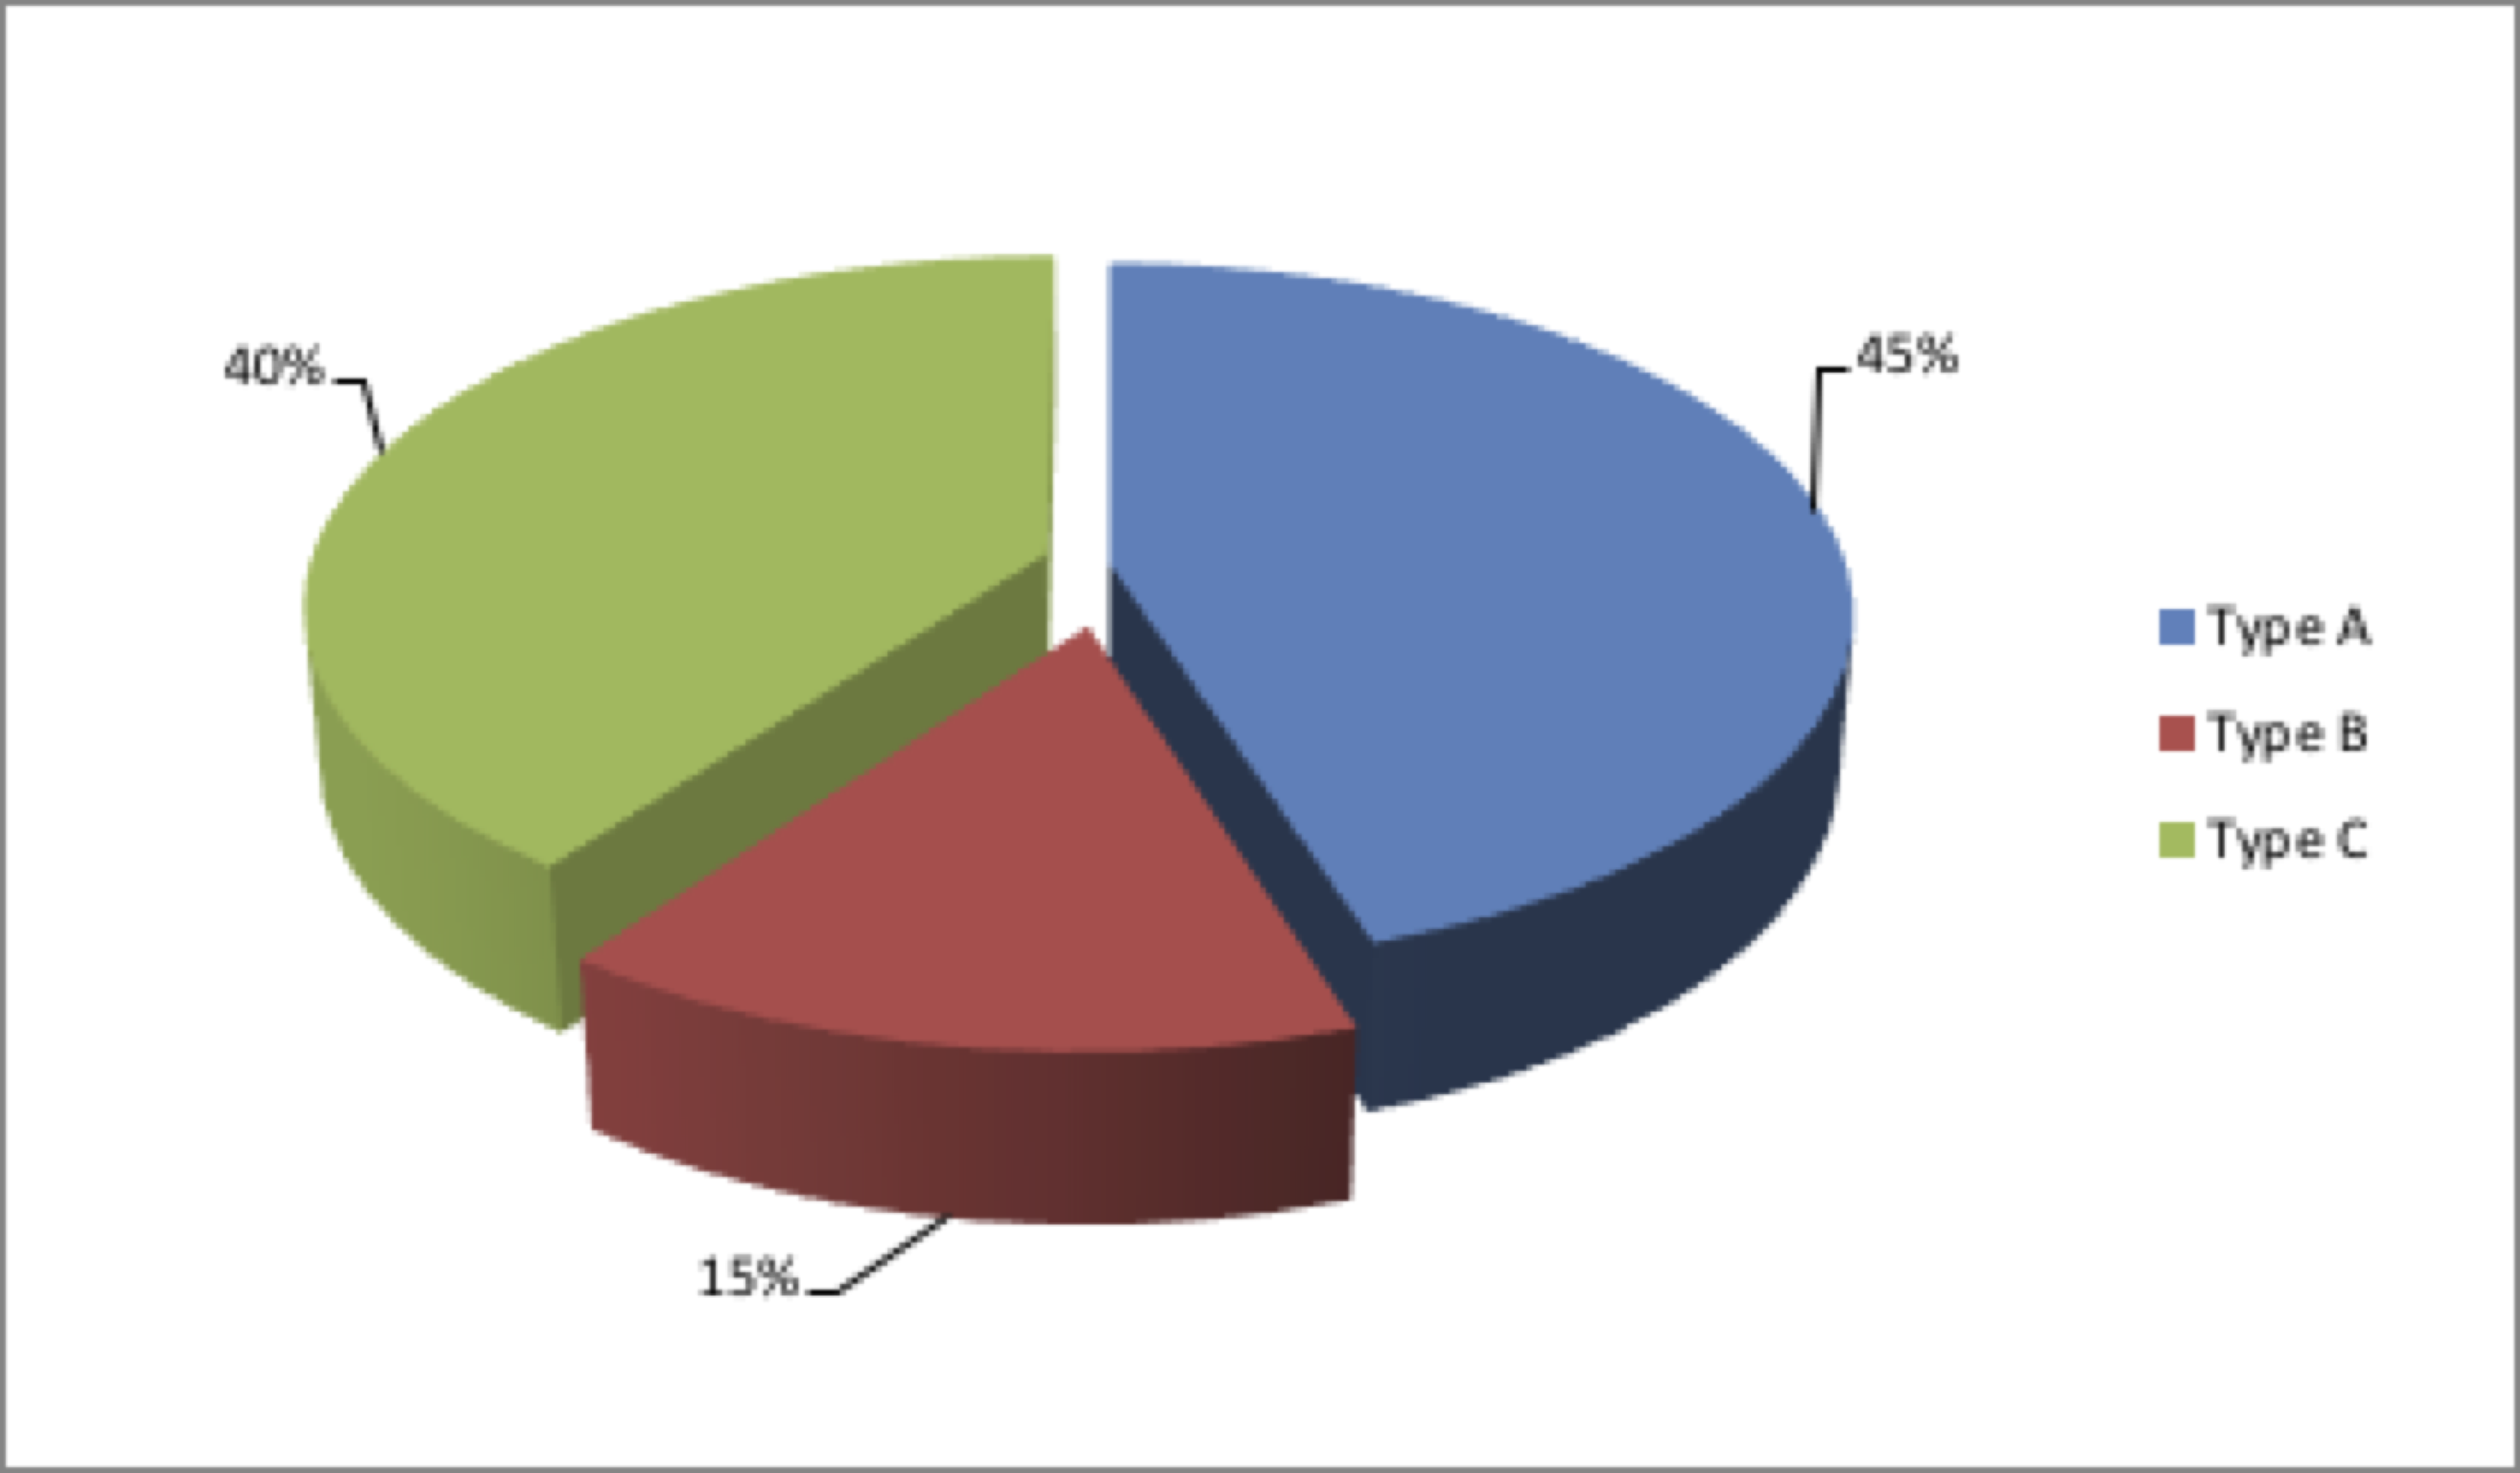
\includegraphics[width=\textwidth]
        {piechart.png}}
       \caption{\label{fig:piechart} EXAMPLE PIE CHART}
\end{figure}

\begin{figure}[!htb]
        \center{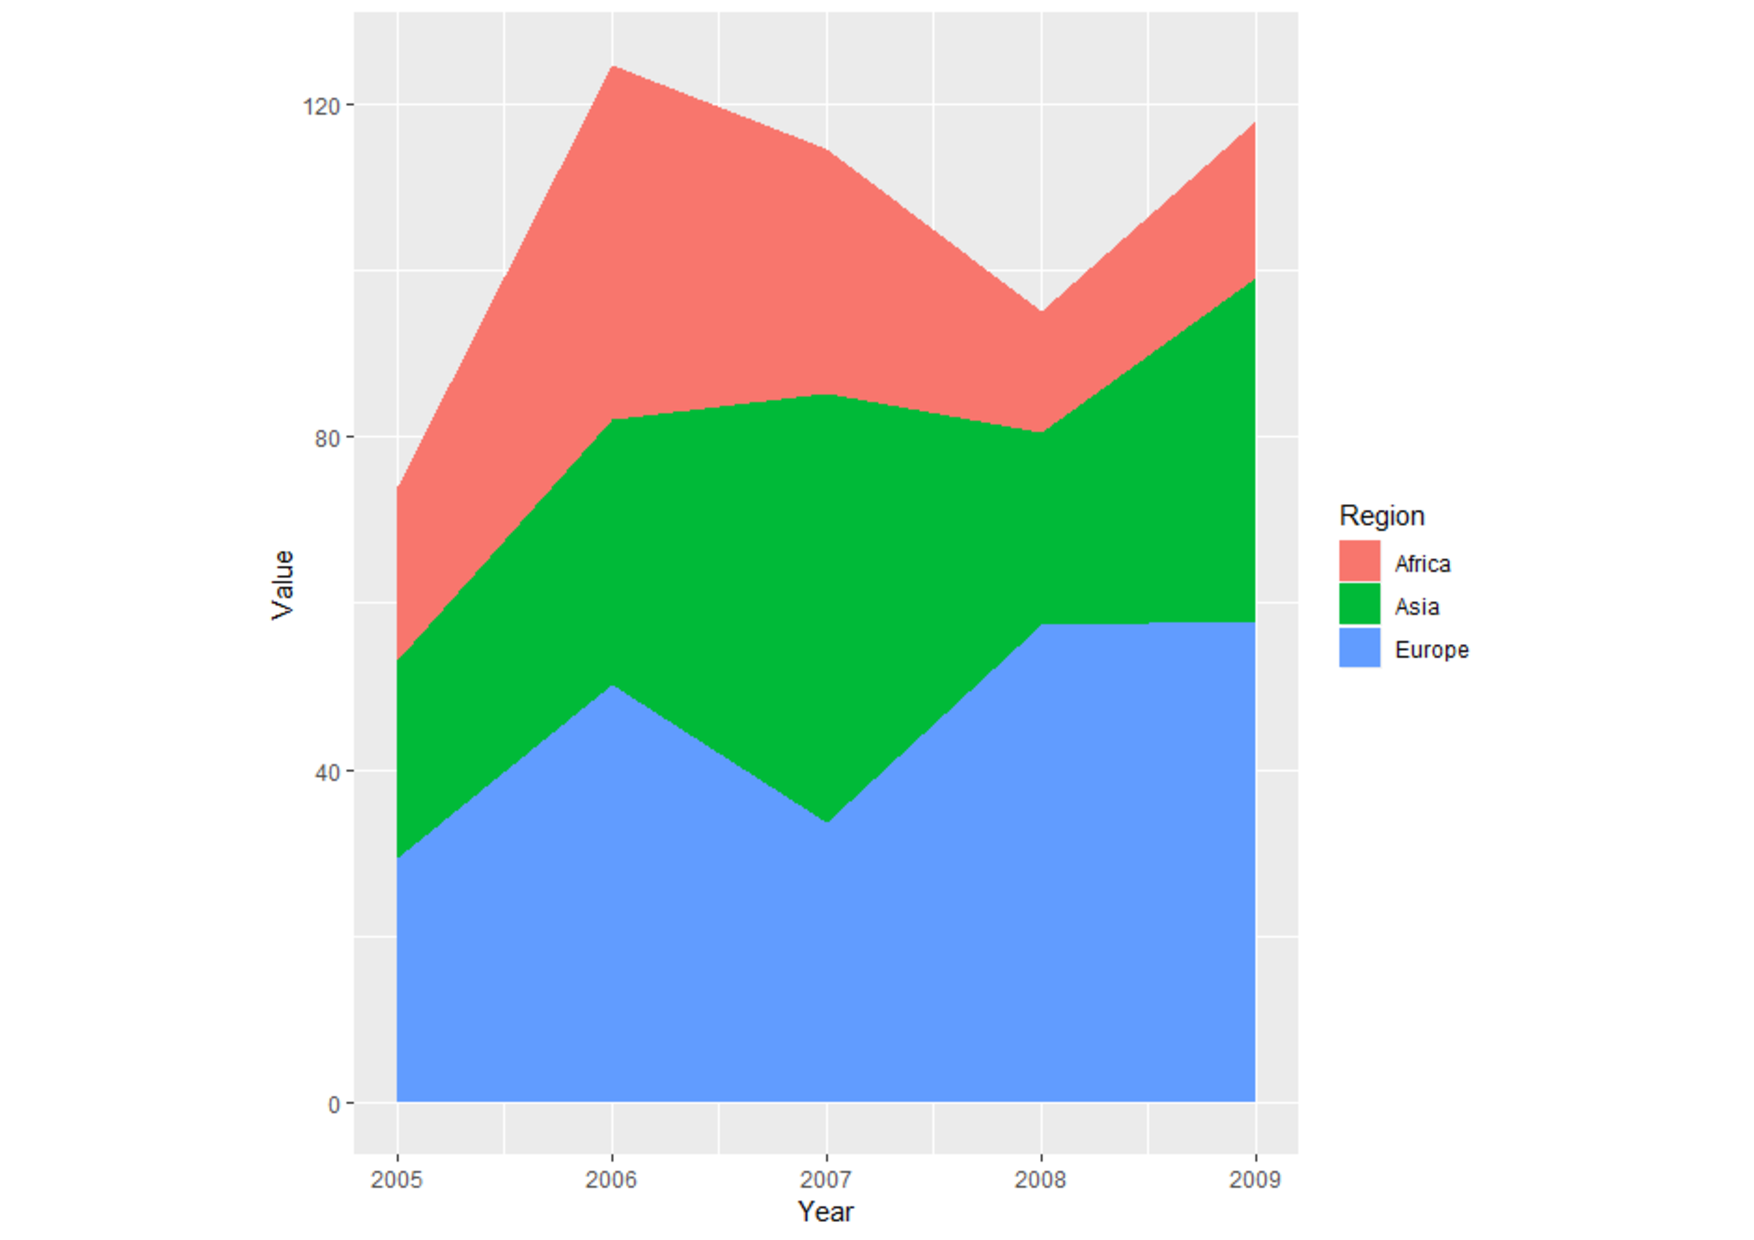
\includegraphics[width=\textwidth]
        {areachart.pdf}}
        \caption{\label{fig:areachart} EXAMPLE AREA CHART}
\end{figure}

\begin{figure}[!htb]
        \center{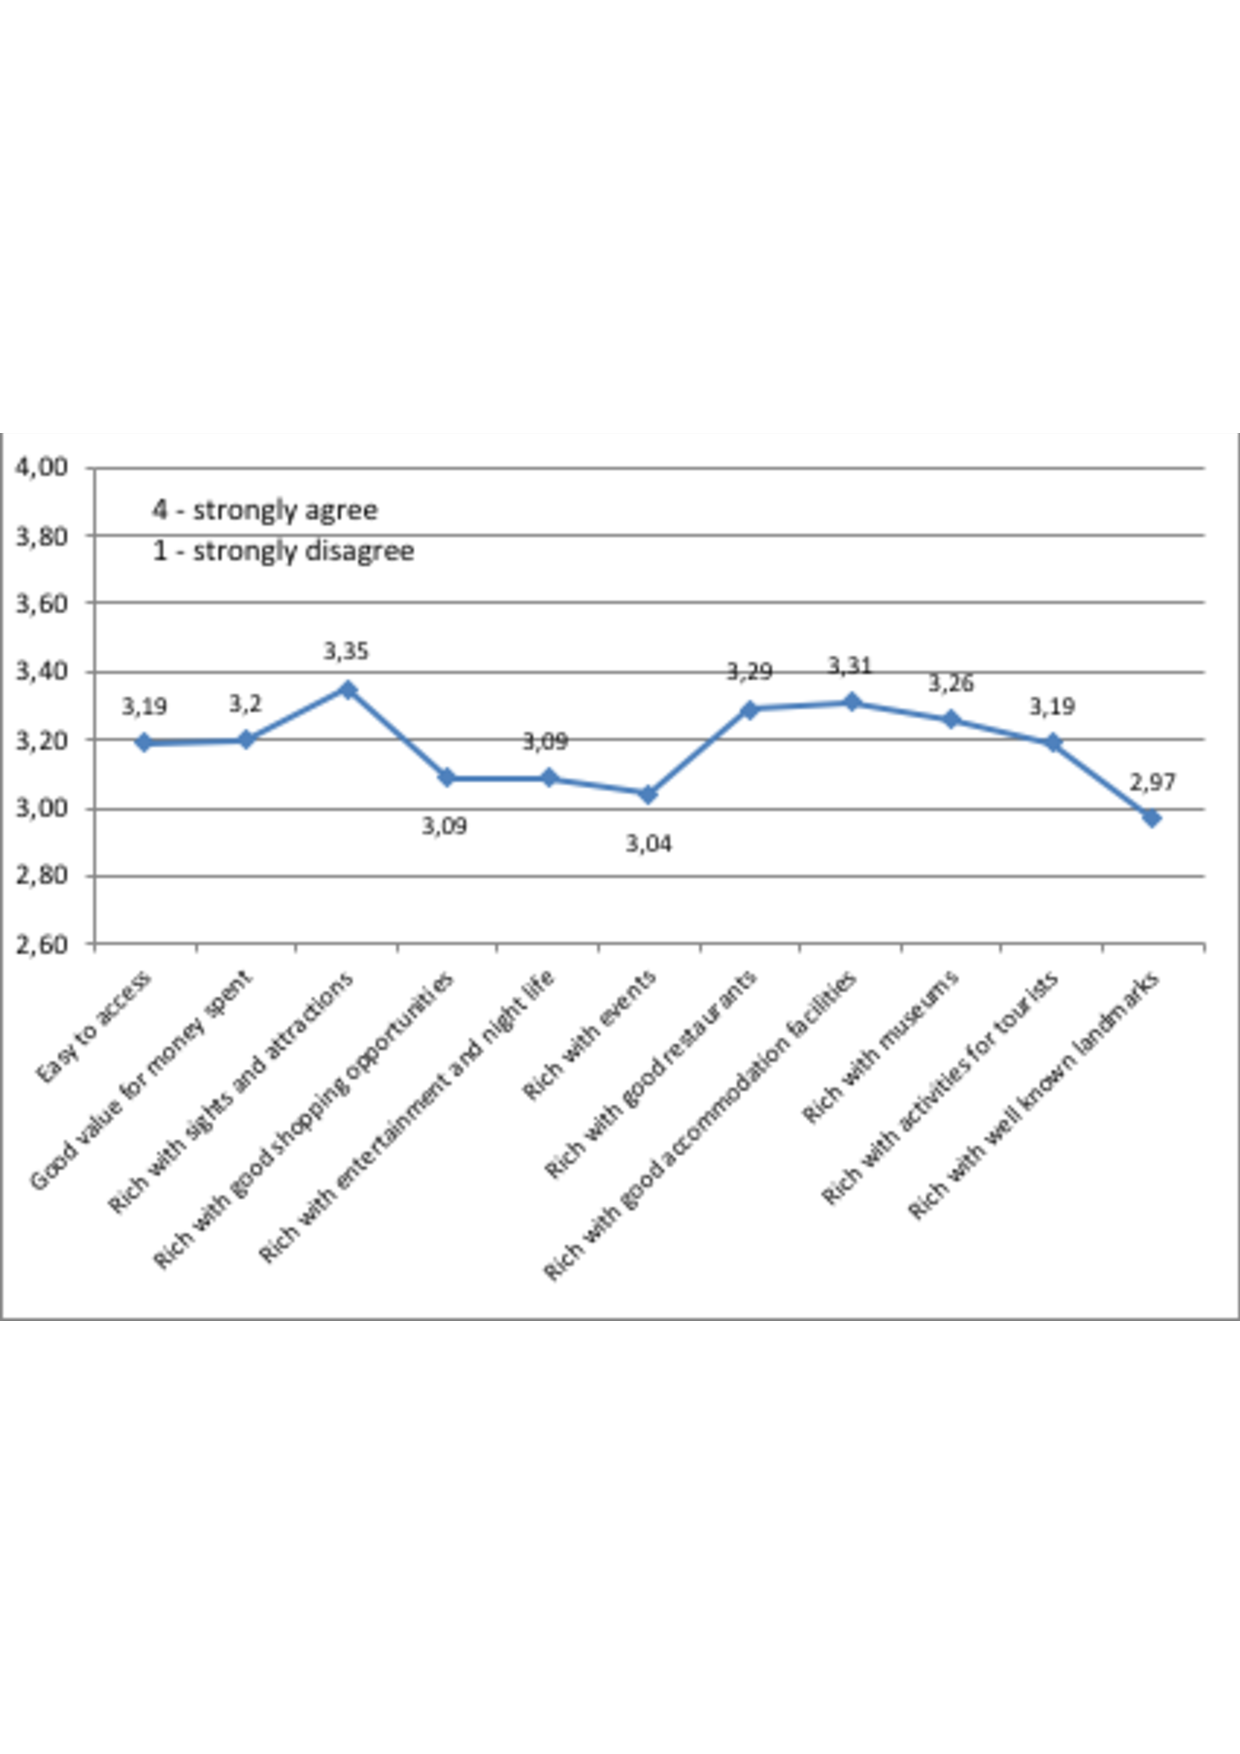
\includegraphics[width=\textwidth]
        {linechart.pdf}}
        \caption{\label{fig:linechart} EVALUATION OF FUNCTIONAL IMAGE ATTRIBUTES, Source: Tsirk, 2009}
\end{figure}      

\section{Qualitative research}
\label{sec:qualitativeresearchs}

This necessitates the use of text description. Although content analysis may produce quantitative results which may be displayed using graphs or tables, quotes from qualitative research are important to support your arguments. 

\subsection{Examples of figures created from content analysis}
 
 \begin{figure}[!htb]
        \center{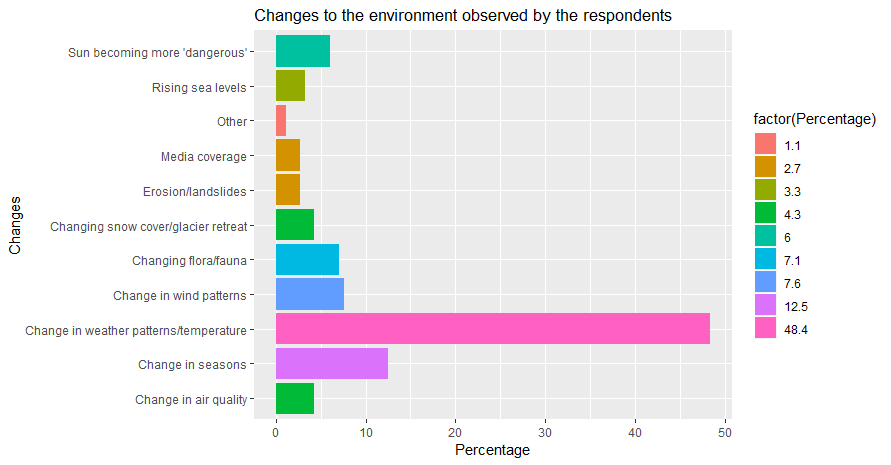
\includegraphics[width=\textwidth]
        {responses.png}}
        \caption{\label{fig:my-label} CHANGES TO THE ENVIRONMENT OBSERVED BY THE RESPONDENTS}
\end{figure}    


\section{Quotations}

“Quotations are statements which have been made explicitly by your respondents.”
“These may be included to highlight specific points that you are making, accompanied by text and interpretation.”

\section{Conclusion}
\label{sec:conclucionchapter4}
Short summary and link to next chapter


         % Results

%----------------------------------------------------------------
%
%  File    :  conclusion.tex
%
%  Author :  Wolfgang Radinger-Peer
% 
%  Created :  3. Feb 2019
% 
%  Changed :  3. Feb 2019
% 
%----------------------------------------------------------------

\chapter{\textsc{Conclusion}}
\label{chap:conclusion}
You can adjust the headings of this section (or avoid them altogether) according to your document structure and findings. 

\section{Summary}
\label{sec:summary}

\section{Contribution to knowledge}
\label{sec:contribution}

\section{Implications for relevant stakeholders}
\label{sec:impact}

\section{Future research}
\label{sec:futurework}
   % Conclusion

% --- Bibliography ------------------------------------------------------

\newpage

%\bibliographystyle{alpha}
%\bibliographystyle{apacitex}
%\bibliography{thesis}

\begin{refsection}[thesis]
	\nocite{*}
\end{refsection}
\printbibliography

%\nocite{*}
%\addcontentsline{toc}{chapter}{Bibliography}

% List references I definitely want in the bibliography,
% regardless of whether or not I cite them in the thesis.


% --- List of Listings -----------------------------------------------------

%\newpage
%\phantomsection
%\addcontentsline{toc}{chapter}{Listings}
%\lstlistoflistings

         % Bibliography

% --- Appendix---------------------------------------
\appendix

%----------------------------------------------------------------
%
%  File    :  appendix.tex
%
%  Authors :  Wolfgang Radinger-Peer
% 
%  Created :  3. Feb 2019
% 
%  Changed :  30 Oct 2008
% 
%----------------------------------------------------------------

\chapter{\textsc{Appendices}}
\label{chap:app}

Appendices contain material that is too large for inclusion in the text or would interrupt the flow of the presentation if it were to be cited in detail. Such texts include the minutes of a meeting, questionnaires, interview outlines and records and the like. References to material in the appendix are indicated by the word appendix and a capital letter beginning with A in the reference sequence in the text. Each appendix begins on a new sheet.

\clearpage

\section{Appendix 1: Financial Market Terms}
bearish
bullish
long
short
	 %  appendix

\end{document}


